\section{Vorgehensweise}\label{sec:vorgehensweise}

\subsection{Stakeholder}\label{subsec:stakeholder}

Am Projekt IP5 Cloudbasiertes Praxisrufsystem sind folgende drei Stakeholder beteiligt.

\subsubsection*{Prof. Daniel Jossen}

\begin{itemize}
    \item Rolle: Auftraggeber und Betreuer
    \item Kontakt: daniel.jossen@fhnw.ch
\end{itemize}

\subsubsection*{Joshua Villing}

\begin{itemize}
    \item Rolle: Student
    \item Kontakt: joshua.villing@students.fhnw.ch
\end{itemize}

\subsubsection*{Kevin Zellweger}

\begin{itemize}
    \item Rolle: Student
    \item Kontakt: kevin.zellweger@students.fhnw.ch
\end{itemize}

\clearpage

\subsection{Projektplan}\label{subsec:projektplan}

\subsubsection*{Übersicht}
\begin{figure}[h]
    \label{fig:projectPlan}
    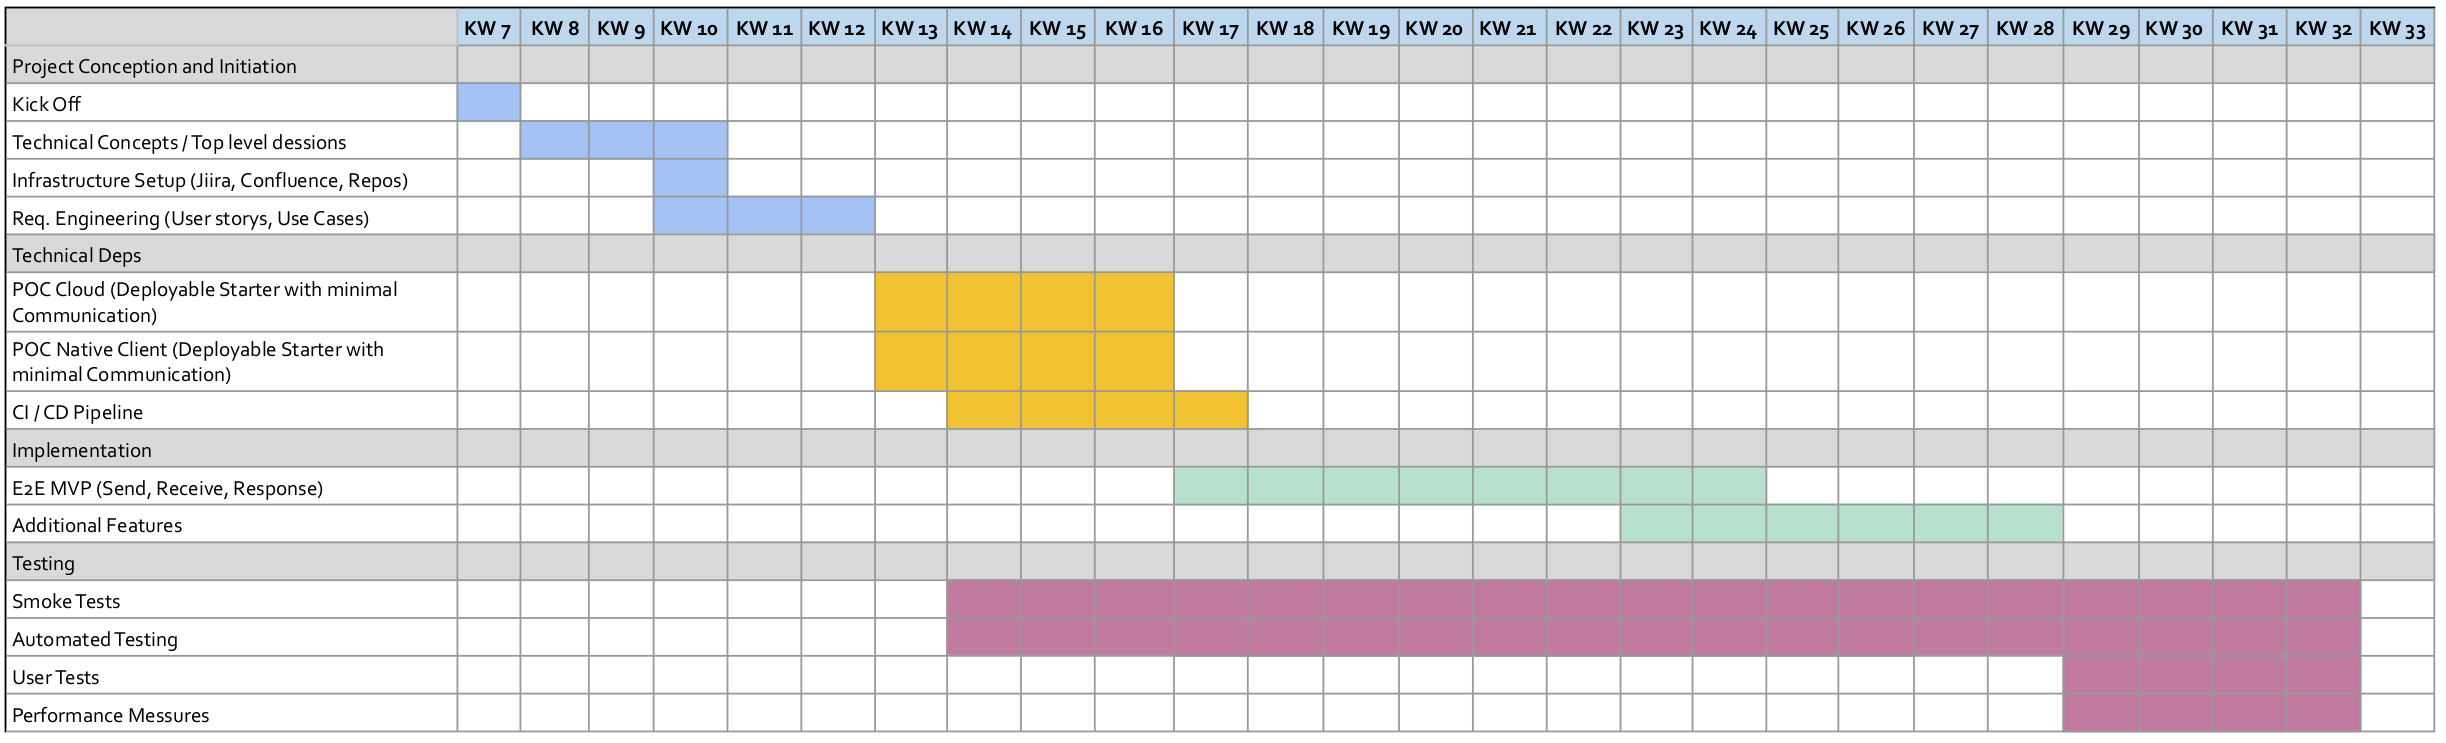
\includegraphics[width=\linewidth]{graphics/Projectplanning}\caption[Projektplan]{Projektplan}
\end{figure}

\subsubsection*{Milestones}

Milestones


POC: Mobile Client -\textgreater Cloud Nachricht schicken und etwas persistieren

Wahrscheinlich über HTTP / Rest


POC: Cloud -\textgreater Mobile Client Nachricht schicken und etwas anzeigen

Wahrscheinlich über Message Broke


Versenden mit hinterlegter Konfiguration


Konfigurierte Notification Types


1:N Versenden, emfpangen und konfigurieren


Setup Wizard (Neu oder z.B. wie Praxiszimmer XY)


Voice to Speech


Voice Chat 1:n (Out Of Scope?)




\clearpage

\subsection{Organisation}\label{subsec:organisation}

\subsubsection*{Kommunikation}

Das Projekt IP5 Cloudbasiertes Praxisrufsystem wurde im FS21 gestartet. Die Organisation und Kommunikation des Projektes mussten dementsprechend für die Einschränkungen wegen Corona angepasst werden.
Um sicherzustellen, dass die Kommunikation über die gesamte Projektdauer funktionieren kann, haben wir uns deshalb von Anfang an entschieden die Kommunikation über Remote- und Online Tools zu organisieren.
Für Besprechungen und Planungen wurde Microsoft Teams gewählt. Die entsprechende Infrastruktur wurde von der FHNW zur Verfügung gestellt.

\subsubsection*{Dokumentation}

Der Bericht wurde mit LateX und zusammen mit dem Quellcode verwaltet. Kurze Besprechungen, Notizen und interne Dokumentation erfolgten über ein geteiltes One Note Notizbuch.

Sämtliche Diagramme, Mockups und Skizzen wurden direkt in den Tools verwaltet, die zur Erstellung gebraucht wurden. Zum Schluss wurden alle für den Bericht relevanten Darstellungen exportiert und in den Bericht integriert.

\subsubsection*{Quellcodeverwaltung}

Sämtlicher Quellcode der im Rahmen des Projektes entsteht, wurde mit Git verwaltet. Der Quellcode ist für Berechtigte unter dem Projekt IP5-Cloudbasiertes-Praxisrufsystem auf github.com einsehbar.
(Referenz https://github.com/IP5-Cloudbasiertes-Praxisrufsystem). Berechtigungen können bei Joshua Villing oder Kevin Zellweger angefordert werden.

\begin{itemize}
    \item IP5-praxis-mobile-client
    \item IP5-praxis-cloud-service
    \item IP5-praxis-admin-ui
    \item IP5-praxis-documentation
\end{itemize}

\subsubsection*{Tools und Werkzeuge}

\begin{itemize}
    \item draw.io
    \item moqus.com
    \item Visual Studio Code
    \item IntelliJ
    \item Git
    \item github.com
\end{itemize}
